\documentclass[11pt]{article}
% --- Encoding e font ---
\usepackage[utf8]{inputenc}
\usepackage[T1]{fontenc}
\usepackage{lmodern}

% --- Matematica ---
\usepackage{amsmath,amssymb,amsfonts,gensymb,amsthm}
\DeclareMathOperator*{\argmin}{arg\,min}
\DeclareMathOperator*{\argmax}{arg\,max}
\usepackage{centernot}
% --- Grafica, colori, float ---
\usepackage{graphicx}
\usepackage[dvipsnames]{xcolor}
\usepackage{float}
% --- Liste e ambienti ---
\usepackage{enumitem}
% --- Caption, numerazione figure ---
\usepackage{caption}
\usepackage{chngcntr}
% --- Caption, numerazione figure ---
\captionsetup{font=small, labelfont=bf, textfont=it}
% --- Indice/TOC personalizzazione (se ti serve) ---
\usepackage{tocloft}
% --- colorbox
\usepackage[most]{tcolorbox}
%--- spazio tra le riga
\usepackage{parskip}
\setlength{\parskip}{0.15cm}
% Elenchi compatti:
\setlist[itemize]{ topsep=2pt, itemsep=0pt, parsep=0pt}
\setlist[enumerate]{topsep=2pt, itemsep=0pt, parsep=0pt}

% Per il codice
\usepackage{listings}
% Definisci i colori esatti di VS Code (tema Light+)
\definecolor{vscodeblue}{RGB}{0,0,255}          % Keywords
\definecolor{vscodeorange}{RGB}{163,21,21}      % Strings
\definecolor{vscodegreen}{RGB}{0,128,0}         % Comments
\definecolor{vscodepurple}{RGB}{197,134,192}    % Control flow e import
\definecolor{vscodeyellow}{RGB}{121,94,38}      % Functions
\definecolor{vscodebg}{RGB}{255,255,255}        % Background
\definecolor{vscodeframe}{RGB}{200,200,200}     % Frame

% Configurazione Python stile VS Code
\lstdefinestyle{vscode}{
    language=Python,
    alsoletter={.},
    backgroundcolor=\color{vscodebg},
    commentstyle=\color{vscodegreen}\itshape,
    numberstyle=\tiny\color{gray},
    stringstyle=\color{vscodeorange},
    basicstyle=\ttfamily\small,
    breakatwhitespace=false,
    breaklines=true,
    captionpos=b,
    keepspaces=true,
    numbers=left,
    numbersep=8pt,
    showspaces=false,
    showstringspaces=false,
    showtabs=false,
    tabsize=4,
    frame=single,
    rulecolor=\color{vscodeframe},
    framesep=10pt,
    xleftmargin=15pt,
    framexleftmargin=15pt,
    % Resetta tutte le keyword e ridefiniscile
    morekeywords={},
    deletekeywords={for,if,while,else,elif,return,break,continue,try,except,finally,with,as,pass,raise,assert,import,from},
    % Keywords blu
    keywordstyle=\color{vscodeblue}\bfseries,
    morekeywords={def,class,lambda,and,or,not,is,in,del,global,nonlocal,yield,await,async,True,False,None,self},
    % Control flow VIOLA
    keywordstyle=[2]\color{vscodepurple}\bfseries,
    morekeywords=[2]{for,if,while,else,elif,return,break,continue,try,except,finally,with,as,pass,raise,assert,import,from},
    % Funzioni
    emph={sqrt,print,input,range,len,str,int,float,list,dict,set,tuple},
    emphstyle=\color{vscodeyellow}
}
\lstset{style=vscode}

%-- for definition (POI definisci defbox)
\newtcolorbox{defbox}[1]{
    colback=gray!10,
    colframe=gray!50,
    fonttitle=\bfseries,
    coltitle=black,
    title=\mbox{#1},  % Cambiato qui
    sharp corners,
    boxrule=0.5pt, breakable}
%-----
%-----
\usepackage{needspace}
%---- Notebox definition \begin{noteboxtitle}{title}
\newtcolorbox{noteboxtitle}[1]{
    colback=white,
    colframe=black!90,
    boxrule=0.8pt,
    arc=3mm,
    title=#1,
    fonttitle=\bfseries,
    left=5pt,
    right=5pt,
    top=5pt,
    bottom=5pt,
      breakable
}

% --- comment
\usepackage{comment}
% --- Margini ---
\usepackage[a4paper,
    top=2.5cm,
    bottom=2.5cm,
    left=2.5cm,
    right=2.5cm,
    bindingoffset=0.5cm
]{geometry}
% --- Titolo con immagine (opzionale) ---
\usepackage{titlepic} % solo se usi \titlepic
% --- Hyperref VA QUASI SEMPRE PER ULTIMO ---
\usepackage{hyperref}
\usepackage{adjustbox}
\usepackage{xltabular}
\usepackage{booktabs}
\raggedbottom


%---Per spezzare le tabelle
\usepackage{longtable}


% --- New structure for Example
\newtheoremstyle{smallexample}
  {3pt}% Space above
  {3pt}% Space below
  {\small}% Body font - testo dell'esempio piccolo
  {}% Indent amount
  {\small\bfseries}% Theorem head font - "Example 18.1" piccolo e grassetto
  {.}% Punctuation after theorem head
  {.5em}% Space after theorem head
  {}% Theorem head spec
\theoremstyle{smallexample}
\newtheorem{example}{Example}[section]
\usepackage[version=4]{mhchem}
\graphicspath{{Images/}}

 %% --- Definizione prima pagina 


%%___NEW COMMAND
\newcommand{\vs}{\vspace{0.2\baselineskip}}



%%%--- Librerie per grafici

\usepackage{tikz}
\usetikzlibrary{positioning, arrows.meta, shapes.geometric, calc}
\usepackage{tcolorbox}
\tcbuselibrary{breakable, skins}



\parindent 0px
\title{\Huge Data Mining and Machine Learning}
\author{\Large Gennaro Basile}
\date{\today}

\titlepic{
    \begin{center}
        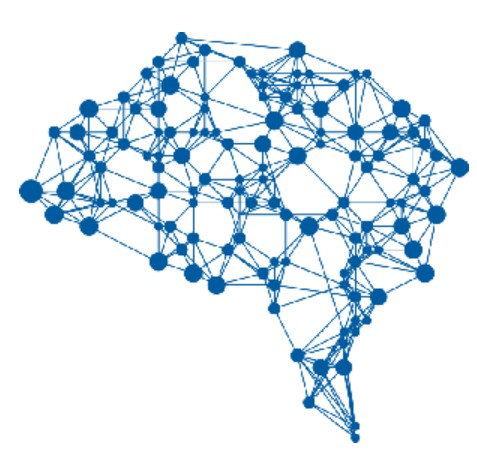
\includegraphics[scale=1]{0.DeepLearningLogo.jpg}
    \end{center}}



\begin{document}
\maketitle
\counterwithin{figure}{subsection}
\captionsetup[figure]{labelfont=bf}

\pagebreak

%% -- Sommario
\tableofcontents
\pagebreak

\begin{itemize}
  \item \textbf{Imputazione multipla} (slide 50--57)
    \begin{itemize}
      \item Single vs Multiple Imputation; MICE (slide 50--51)
      \item Come funziona MICE: FCS, Gibbs Sampler, flessibilità modulare (slide 52--55)
      \item Pooling con le Regole di Rubin (slide 56)
      \item Pro e contro di MICE (slide 57)
    \end{itemize}

  \item \textbf{Imputazione nel paradigma Statistical Learning} (slide 58--66)
    \begin{itemize}
      \item Nuovo paradigma: imputazione come supervised learning (slide 58--59)
      \item Incremental Tree-Based Imputation e lexicographic ordering (slide 60--61)
      \item Boosting e algoritmo BINPI (slide 62--64)
      \item Pseudo-codice BINPI-MISSING (slide 65)
      \item Simulazioni e confronto tra metodi (slide 66--69)
    \end{itemize}

  \item \textbf{Data Fusion} (slide 70--72)
    \begin{itemize}
      \item Meccanismo Donor/Receptor file, variabili comuni e specifiche
      \item Pseudo-codice BINPI-FUSION
    \end{itemize}

  \item \textbf{Imbalanced response: generazione di dati sintetici} (slide 73)
    \begin{itemize}
      \item SMOTE e varianti (SMOTE-ENN, SMOTE-TL, ADASYN, Borderline-SMOTE, ROSE, \ldots)
    \end{itemize}

  \item \textbf{Data Transformation} (slide 74)
    \begin{itemize}
      \item Smoothing, feature construction, aggregazione, normalizzazione,
            discretizzazione, recoding
    \end{itemize}

  \item \textbf{Scaling e Normalizzazione} (slide 75)
    \begin{itemize}
      \item Standardizzazione (z-score) e Min-Max scaling
    \end{itemize}

  \item \textbf{Data Reduction: motivazioni e tassonomia} (slide 76)
    \begin{itemize}
      \item Obiettivi (spazio, tempo, rumore, strutture nascoste, manifold learning)
      \item Quattro approcci: Sampling, Feature Subset, Axis Rotation, Type Transformation
    \end{itemize}

  \item \textbf{Sampling} (slide 77--79)
    \begin{itemize}
      \item Unbiased (con/senza rimpiazzo), biased (temporal-decay), stratified (slide 77--78)
      \item Reservoir sampling per data stream (slide 79)
    \end{itemize}

  \item \textbf{Feature Subset Selection} (slide 80)
    \begin{itemize}
      \item Unsupervised (clustering-guided) e supervised (classification-guided)
    \end{itemize}

  \item \textbf{Dimensionality Reduction con Axis Rotation} (slide 81)
    \begin{itemize}
      \item PCA e SVD come metodi per rimuovere correlazioni e ridurre dimensionalità
    \end{itemize}
\end{itemize}

\pagebreak



\section{Data Preparation}

\subsection{Introduction and Motivation}

\subsubsection{The Golden Rule: GIGO}

The foundational principle of Data Science is \textbf{GIGO (Garbage In -- Garbage Out)}. No machine learning algorithm, regardless of its complexity, can extract correct insights from flawed data. Data preparation is the mandatory phase that bridges raw, chaotic data and analytical modeling.

Real-world data suffers from three primary defects:
\begin{itemize}
    \item \textbf{Incompleteness}: Missing values or absent features.
    \item \textbf{Inaccuracy (Noise)}: Sensor faults, data-entry errors, or out-of-range values.
    \item \textbf{Inconsistency}: Discrepancies in coding across different merged databases.
\end{itemize}

\subsubsection{Why Data Needs to Be Pre-processed}


  \textbf{Data preparation} (also called \emph{data pre-processing}) is the set of operations
  applied to raw data before analysis, aimed at making the data suitable for mining algorithms.
  It is necessary because data from different sources is heterogeneous, often unstructured (e.g.,
  raw logs), and requires feature extraction before it can be fed into an algorithm.

\vs

\textbf{Key Issues in Data Preparation}

Eight key questions guide the data preparation process:

\begin{itemize}
  \item \textbf{Data Cleansing} -- \textit{How do I clean up the data?}
        Detect and correct errors, resolve inconsistencies.


  \item \textbf{Data Transformation} -- \textit{How do I express the variables?}
        Choose appropriate scales, encodings, and representations.

  \item \textbf{Data Imputation} -- \textit{How do I handle missing values?}
        Apply statistical methods (mean substitution, regression imputation, multiple
        imputation, etc.) to estimate absent entries.

  
  \item \textbf{Data Weighting} -- \textit{Are all cases treated the same?}
        Decide whether some records should carry higher importance (e.g., oversampling of
        rare classes).

  
  \item \textbf{Data Filtering} -- \textit{What do I do about outliers and other unwanted data?}
        Identify and handle extreme or erroneous observations that may distort the analysis.

 
  \item \textbf{Data Abstraction} -- \textit{How do I handle temporal data?}
        Aggregate, resample, or extract features from time-stamped records.

  
  \item \textbf{Data Reduction} -- \textit{Can I reduce the amount of data to use?}
        Apply dimensionality reduction (PCA, SVD) or instance selection to shrink the dataset
        while preserving its informational content.

 
  \item \textbf{Data Derivation} -- \textit{Can I create some new variables?}
        Engineer new features that capture domain knowledge or improve predictive power.
\end{itemize}

\subsubsection{Data Cleaning vs. Data Cleansing}

Though often used interchangeably, distinguishing these two operations is critical for a robust pipeline:
\begin{itemize}
    \item \textbf{Data Cleaning} (Automated/Syntactic): Surface-level fixes like dropping duplicate rows, standardizing date formats, or simple mean imputation.
    \item \textbf{Data Cleansing} (Manual/Semantic): Deep validation requiring a \textbf{domain expert}. It involves cross-referencing external knowledge to fix logical contradictions that an algorithm wouldn't catch.
\end{itemize}


\subsubsection{Feature Extraction and Computational Constraints}

A fundamental practical issue in data mining is that algorithms are constrained by
\textbf{main memory}. Consider K-means clustering:

\begin{itemize}
  \item Clustering $\tfrac{1}{4}$ GB of data: $\approx 100$ seconds.
  \item Clustering $1$ GB of data: $\approx 400$ seconds.
  \item Clustering $1.1$ GB of data (exceeds RAM): \emph{several hours}.
\end{itemize}

\noindent When the dataset exceeds main memory, the algorithm is forced to swap data to disk,
causing a catastrophic increase in execution time. This motivates \textbf{data reduction}
techniques that create compact, memory-resident representations of the data while preserving
the essential structure. 


\begin{defbox}{Feature Extraction}
  \textbf{Feature extraction} is the process of transforming raw data into a set of
  informative, non-redundant features suitable for a given mining task. It is as much an
  \emph{art} as a science: the quality of the extracted features determines an upper bound on
  the quality of any subsequent analysis.
\end{defbox}



When data types don't match the algorithm's requirements, we must apply:

\begin{defbox}{Data Type Portability}
  \textbf{Data type portability} refers to the process of converting data from one
  representation type to another so that it can be processed by a specific algorithm or
  integrated into a unified pipeline.
\end{defbox}

\noindent Key principles:
\begin{itemize}
  \item The choice of features and their representation must be tailored to the task.
  \item A \textbf{domain expert} must be consulted: domain knowledge is irreplaceable for
        identifying which signals are meaningful.
  \item If the correct features are not extracted, the analysis can only be as good as the
        available raw data -- no algorithm can recover information that was never captured.
\end{itemize}

\subsubsection{Data Type Conversions}

\begin{enumerate}
\item\textbf{Numeric to Categorical (Discretization / Binning)}.
Continuous variables are split into $k$ discrete bins. This is essential for algorithms like Decision Trees or Association Rule Mining.
\begin{itemize}
    \item \textbf{Equi-width}: Bins of equal length. Highly sensitive to skewed data and outliers.
    \item \textbf{Equi-log}: Exponentially spaced boundaries. Ideal for features spanning multiple orders of magnitude (e.g., income).
    \item \textbf{Equi-depth (Quantile)}: Each bin contains the exact same number of records. Highly robust to skewness.
\end{itemize}

\vspace{0.25cm}
\item\textbf{Categorical to Numeric (Binarization)}.
Machine learning models (like Neural Networks or Logistic Regression) require numbers, not text labels. 
\begin{itemize}
    \item \textbf{Binary}: Encode as $\{0, 1\}$ or $\{-1, +1\}$ (the latter is better for SVMs as it centers the data).
    \item \textbf{One-Hot Encoding}: For $K$ categories, create a $K$-dimensional indicator vector. For example, the 2nd category out of 4 becomes $(0, 1, 0, 0)$. This strictly avoids giving the algorithm a false sense of mathematical order (which happens if you just encode them as 1, 2, 3, 4).
\end{itemize}

\vspace{0.25cm}
\item \textbf{Text to Numeric (NLP Processing)}.
Raw text must be converted into a Document-Term Matrix.
\begin{itemize}
    \item \textbf{Cleaning}: Tokenization, Stop Word Removal (dropping "the", "is"), and Stemming (reducing "running" to "run").
    \item \textbf{TF-IDF Weighting}: You must penalize words that appear everywhere and reward rare, highly discriminative words. The weight of term $t$ in document $d$ is:
    \[
        \text{TF-IDF}(t, d) = \text{TF}(t,d) \times \log\!\left(\frac{N}{\text{DF}(t)}\right)
    \]
    where $N$ is total documents and $\text{DF}(t)$ is the number of documents containing $t$.
    \item \textbf{Latent Semantic Analysis (LSA)}: Applies Singular Value Decomposition (SVD) to the sparse matrix to compress it into a dense, lower-dimensional space.
\end{itemize}
\end{enumerate}

\vs
\begin{defbox}{Cosine Similarity for Text}
    In high-dimensional text spaces, Euclidean distance is useless (curse of dimensionality). Always use \textbf{Cosine Similarity}, which measures the angle between two document vectors regardless of their length:
    \[
        \cos(\mathbf{d}_i, \mathbf{d}_j) = \frac{\mathbf{d}_i \cdot \mathbf{d}_j}{\|\mathbf{d}_i\|\,\|\mathbf{d}_j\|}
    \]
\end{defbox}



    \subsection{Time Series Analysis}

\subsubsection{Definition and Core Differences}

\begin{defbox}{Time Series}
    A \textbf{time series} is an ordered sequence of data points measured at successive, uniformly spaced time steps:
    \[
        \mathbf{x} = (x_1,\, x_2,\, \ldots,\, x_T), \quad x_t \in \mathbb{R}
    \]
\end{defbox}

         \begin{figure}[H] 
        \centering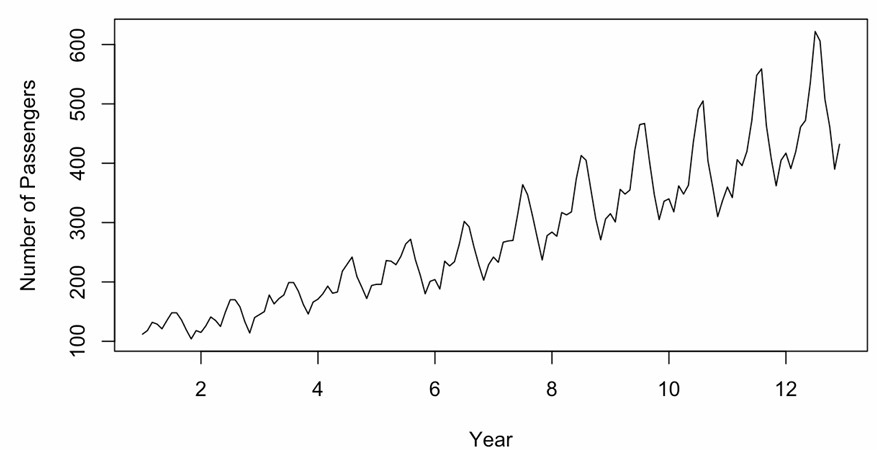
\includegraphics[scale=0.65]{4.Airline Time Series.jpg}
        \caption{Airline Passengers Time Series}
    \captionsetup{font=footnotesize}
    \end{figure}

 Time series break the fundamental assumption of standard Machine Learning because observations are \textit{not} independent and identically distributed (i.i.d.). They are \textbf{autocorrelated}, meaning the temporal order itself is the most informative feature.

\subsubsection{The 7 Classical Time Series Problems}

Working with time series usually boils down to one of these engineering tasks:

\begin{itemize}
    \item \textbf{Join}: Linking similar time series across two different databases (e.g., syncing IoT temperature and humidity sensors).
    \item \textbf{Annotation}: Labeling specific segments of a series.
    \item \textbf{Query by Content}: Finding the $k$ most similar historical trajectories to a current query.
    \item \textbf{Clustering}: Unsupervised grouping of series with similar shapes or seasonalities.
    \item \textbf{Classification}: Supervised prediction of a category based on the series shape.
    \item \textbf{Anomaly Detection}: Finding subsequences that deviate from expected behavior. 
    \item \textbf{Motif Finding}: Identifying the most frequently recurring subsequences (patterns) to understand underlying system dynamics.
\end{itemize}

\subsubsection{SAX: Symbolic Aggregate approXimation}

Machine Learning algorithms for text (like NLP or regex search) are incredibly fast. \textbf{SAX} is the industry standard for converting heavy, continuous time series into lightweight, discrete text strings so we can use those fast algorithms.

It operates in two sequential steps:

\begin{enumerate}
    \item \textbf{PAA (Piecewise Aggregate Approximation)}: Dimensionality reduction. 
    \begin{itemize}
        \item Divide the series of length $T$ into $\omega$ equal-sized windows.
        \item Calculate the mathematical mean of each window. 
        \item You just compressed $T$ points into $\omega$ points.
    \end{itemize}
    \item \textbf{Gaussian Discretization}: 
    \begin{itemize}
        \item Normalize the PAA values to a standard Gaussian distribution (z-score).
        \item Slice the bell curve into $\alpha$ regions of \textit{equal area} (equi-depth).
        \item Map each PAA mean to the letter assigned to its region (e.g., $\Sigma = \{a, b, c, d\}$).
        \item \textbf{Result}: A string like \texttt{baabccbc}.
    \end{itemize}
\end{enumerate}

\subsubsection{Distance Measures and the Lower-Bounding Property}

To compare two time series $Q$ and $C$, the standard metric is \textbf{Euclidean Distance}:
\[
    D(Q, C) = \sqrt{\sum_{i=1}^{n} (q_i - c_i)^2}
\]
However, calculating this on millions of raw data points is computationally impossible in real-time. We use PAA and SAX distances as approximations.

         \begin{figure}[H] 
        \centering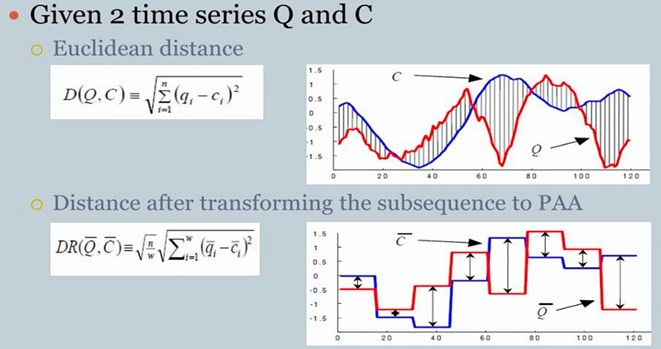
\includegraphics[scale=0.8]{5.Distance Measure.jpg}
        \caption{Distance Measure}
    \captionsetup{font=footnotesize}
    \end{figure}

\begin{defbox}{The Lower-Bounding Property}
    The defining feature of a good approximation distance (like PAA distance) is that it mathematically \textbf{lower-bounds} the true Euclidean distance:
    \[
        DR(\bar{Q}, \bar{C}) \leq D(Q, C)
    \]
    \textbf{Why this matters}: It guarantees \textit{no false dismissals}. If you query a massive database, you can use the cheap PAA distance to quickly filter out bad matches. Because PAA is strictly less than or equal to the true distance, you are mathematically guaranteed never to accidentally filter out the true nearest neighbor.
\end{defbox}

\subsubsection{Applications of SAX}

SAX finds application across a wide variety of domains that involve large-scale time series:

\begin{itemize}
  \item \textbf{Time series analysis}: similarity search, classification, clustering,
        and motif discovery in finance, healthcare, environmental monitoring, and
        telecommunications.
  \item \textbf{Pattern recognition}: identifying recurring patterns or motifs within
        time series to detect similarities and anomalies, enabling better understanding and
        prediction of future behaviour.
  \item \textbf{Anomaly detection}: highlighting deviations from normal symbolic
        patterns, enabling early detection of faults or unusual events (e.g., industrial
        sensor monitoring).
  \item \textbf{Data compression} -- representing long time series with a compact string
        over a small alphabet reduces storage requirements while preserving the essential
        structure needed for analysis.
  \item \textbf{Predictive maintenance} -- in manufacturing and utilities, SAX analyses
        sensor data to detect symbolic patterns indicative of impending equipment failure,
        enabling proactive intervention and reducing downtime.
\end{itemize}

\noindent \textbf{Integration note.} The discrete symbolic representation produced by SAX
opens the door to the rich toolbox of \emph{sequential pattern mining}: algorithms
originally designed for text or DNA sequences (e.g., Apriori-based sequence mining,
suffix arrays, variable-length Markov models) can be directly applied to time series after
SAX transformation.


\subsubsection{Time Series Portability (Dimensionality Reduction)}

When building pipelines (especially distributed ones using Spark or Kafka), you must compress time series into memory-resident forms. The 5 canonical methods are:

\begin{itemize}
    \item \textbf{DFT (Discrete Fourier Transform)}: Maps series to sinusoidal frequencies. Great for highly periodic data; naturally discards high-frequency noise.
    \item \textbf{DWT (Discrete Wavelet Transform)}: Multi-resolution analysis. Unlike DFT, it captures both frequency \textit{and} localized time events (e.g., sudden spikes).
    \item \textbf{SVD (Singular Value Decomposition)}: Matrix-level compression. Extracts the top-$k$ dominant patterns across an entire dataset of multiple series.
    \item \textbf{PLA (Piecewise Linear Approximation)}: Represents the series as connected line segments (slopes and intercepts). Highly interpretable.
    \item \textbf{PAA (Piecewise Aggregate Approximation)}: The mean-based chunking method used in SAX. The fastest and most computationally efficient.
\end{itemize}

\subsection{Frequency-Domain Transformations and Data Conversions}

\subsubsection{Moving from Time to Frequency}


Many real-world data sources are recorded as sequences evolving over time or
space. Before feeding them into standard machine-learning pipelines, they must
be converted into a fixed-size numeric (multidimensional) representation. Two
classical tools for this are the \textbf{Discrete Wavelet Transform (DWT)} and
the \textbf{Discrete Fourier Transform (DFT)}.

\begin{defbox}{Discrete Wavelet Transform (DWT)}
  The DWT converts a time series into a set of \emph{wavelet coefficients} that
  capture averaged differences between different portions of the signal at
  multiple scales. Each coefficient encodes both frequency and localised time
  information, yielding a compact multidimensional representation of the
  original series.
\end{defbox}

\begin{defbox}{Discrete Fourier Transform (DFT)}
  The DFT decomposes a time series into a weighted sum of sinusoids of
  increasing frequency. The resulting frequency coefficients are
  \emph{less dependency-oriented} than the raw time-domain values, making them
  more suitable as features for data-mining tasks such as similarity search and
  classification.
\end{defbox}

For \textbf{spatial series} (two-dimensional contextual features, e.g.\ images),
the same philosophy applies, but the DWT must be adapted to handle two spatial
dimensions simultaneously.





         \begin{figure}[H] 
        \centering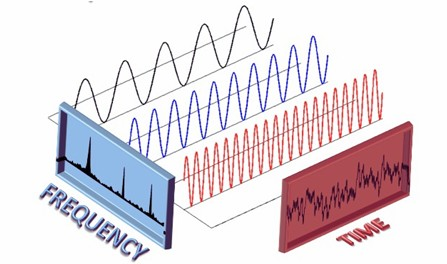
\includegraphics[scale=0.8]{6.Discrete Fourier Transform.jpg}
        \caption{Discrete Fourier Transform}
    \captionsetup{font=footnotesize}
    \end{figure}

    
A signal can be described in two complementary ways:

\begin{itemize}
  \item \textbf{Time domain}: the raw amplitude of the signal at each instant.
        Useful for understanding \emph{how} the signal evolves over time, but
        not ideal for extracting frequency content.

  \vspace{0.2cm}
  \item \textbf{Frequency domain (spectrum)}: the signal is expressed as a
        superposition of sinusoids; each sinusoid is characterised by its
        frequency and amplitude. This representation makes frequency content
        immediately visible and is the output of the Fourier Transform.
\end{itemize}


\subsubsection{Spectrograms and Human Perception}  

\begin{defbox}{Spectrum}
  A \emph{spectrum} is a representation of a signal's frequency content. It
  shows how the amplitude (energy or power) of the signal is distributed across
  different frequencies. Every point on the frequency spectrum represents the
  power or amount of energy present at that frequency over a finite time window.
\end{defbox}

Instead of looking at a simple 1D line chart, Data Scientists often convert time series into 2D images called \textbf{Spectrograms}. Time is on the x-axis, frequency is on the y-axis, and color intensity represents energy. This allows you to feed time-series data directly into powerful image-recognition models (like CNNs).


  \begin{itemize}
    \item \textbf{White/light regions}: silence or low energy at that frequency.
    \item \textbf{Dark regions}: high energy caused by vibration in the signal.
  \end{itemize}



\noindent\textbf{Why spectrograms matter for data mining}: a spectrogram converts a
1-D time series into a 2-D image-like representation; image-based feature
extractors (e.g.\ convolutional neural networks) can then be applied directly.

         \begin{figure}[H] 
        \centering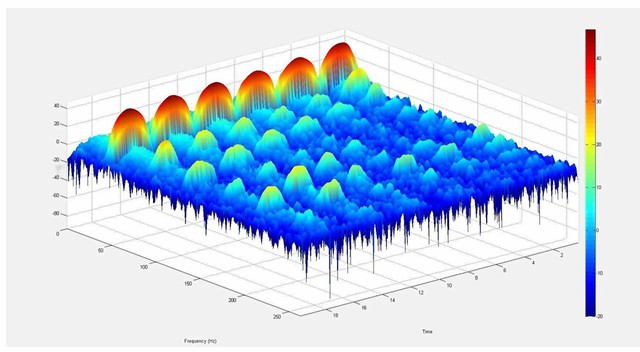
\includegraphics[scale=0.7]{7.Spectrogram.jpg}
        \caption{Spectrogram}
    \captionsetup{font=footnotesize}
    \end{figure}

        Human hearing is non-linear: we easily distinguish between 100Hz and 200Hz, but cannot tell the difference between 10,000Hz and 10,100Hz.

\begin{defbox}{The Mel Scale and Spectrogram}
    The \textbf{Mel Scale} warps physical frequencies to match human perception:
    \[
        m = 2595\,\log_{10}\!\left(1 + \frac{f}{700}\right)
    \]
    A \textbf{Mel Spectrogram} is the absolute industry standard feature representation for any audio Machine Learning task (e.g., speech recognition, genre classification).
\end{defbox}

             \begin{figure}[H] 
        \centering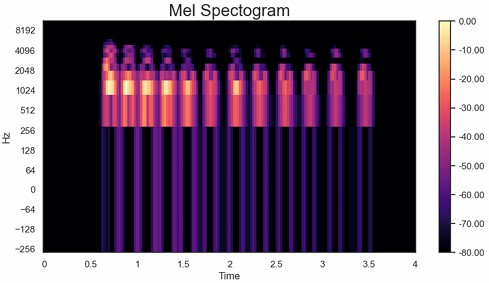
\includegraphics[scale=0.7]{9.Mel Spectrogram.jpg}
        \caption{Mel Spectrogram}
    \captionsetup{font=footnotesize}
    \end{figure}

\subsubsection{Converting Sequences and Graphs to Numeric Data}

Standard ML algorithms need fixed-size number arrays, not strings or networks.

\begin{itemize}
    \item \textbf{Discrete Sequences}: For a sequence of categorical symbols (e.g., DNA like \texttt{ACACACTG} or user-click paths), you first binarize the sequence (one-hot encoding over time). Then, you apply a Wavelet Transform (DWT) to each binary array. The resulting coefficients capture both how often a symbol appears and its positional locality.
    \vs

    \item \textbf{Graphs}: 
    \begin{itemize}
        \item \textbf{MDS (MultiDimensional Scaling)}: Projects nodes into a Euclidean space while preserving their pairwise distances.
        \item \textbf{Spectral Transformation}: Analyzes the eigenspectrum of the Graph Laplacian matrix ($\mathbf{L} = \mathbf{D} - \mathbf{W}$). The eigenvectors corresponding to the smallest eigenvalues create a low-dimensional embedding of the network's structure.
    \end{itemize}
\end{itemize}

\subsubsection{The Universal Solution: Similarity Graphs}

If your data is too chaotic (mixed text, images, coordinates), you can convert \textit{anything} into a \textbf{Neighborhood Graph}. 
\begin{itemize}
    \item \textbf{Nodes}: Your data objects (e.g., users, study locations, documents).
    \item \textbf{Edges}: Connected only if objects are similar (using an $\varepsilon$-radius or $k$-Nearest Neighbors).
    \item \textbf{Weights}: Calculated using a \textbf{Heat Kernel}, which forces the weight to exponentially decay as distance increases:
    \[
        W_{ij} = e^{-\dfrac{d(O_i,\,O_j)^2}{t^2}}
    \]



\end{itemize}
Once you have this graph, you can run clustering or anomaly detection regardless of what the original raw data looked like.

\subsection{Data Cleaning, Quality, and Governance}

\subsubsection{The Reality of Dirty Data}
In production systems, data is always flawed. Sensors drift, users lie on forms to protect privacy, data-entry typos occur, and pipeline drops happen. 

\begin{defbox}{Data Governance and DQM}
    \textbf{Data Governance} establishes the authority and policies over a company's data (who can access what). 
    \textbf{Data Quality Management (DQM)} is the active execution of those policies to ensure data is \textit{fit for consumption.} Proper DQM guarantees transparency, standardization, and regulatory compliance.
\end{defbox}

\subsubsection{The Six Dimensions of Data Quality}

When building a robust data pipeline (e.g., streaming logs through Kafka for downstream analytics), you must validate your data against these six independent dimensions:

\begin{itemize}
    \item \textbf{Accuracy}: Does the data correctly reflect reality? (e.g., A temperature reading of 200°C in a server room is syntactically valid as a number, but physically inaccurate).
    \item \textbf{Completeness}: Are there nulls or missing values? (e.g., missing timestamps).
    \item \textbf{Consistency}: Are there contradictions across merged databases? (e.g., User marked as \textit{Active} in the CRM but \textit{Deleted} in the app backend).
    \item \textbf{Timeliness}: Is the data fresh enough to be useful? (A massive delay in log processing renders the data useless for real-time anomaly detection).
    \item \textbf{Validity}: Does it conform to the required format/syntax? (e.g., Dates must be \texttt{YYYY-MM-DD}).
    \item \textbf{Uniqueness}: Are there duplicate records skewing your counts?
\end{itemize}

\subsection{Data Editing and Missing Values}

\subsubsection{Data Editing}

Before handling missing values, data must be logically verified. \textbf{Data Editing} is the automated process of finding and fixing missing, unusual, or logically impossible values with minimal modification to the raw data.
\begin{itemize}
    \item \textbf{Micro-Editing}: Row-level inspection (e.g., checking if a single engine temperature reading is physically impossible).
    \item \textbf{Macro-Editing}: Dataset-level inspection (e.g., checking if the aggregated global average temperature suddenly spiked, indicating a systemic error).
\end{itemize}

\subsubsection{The 3 Missing Data Mechanisms}

Understanding \textit{why} data is missing dictates how you must fix it. You cannot apply imputation blindly. There are three formal mechanisms:


\begin{defbox}{1. MCAR (Missing Completely At Random)}
    The missingness is a coin flip. It is entirely unrelated to the variable itself or any other variable in the dataset.
    \begin{itemize}
        \item \textbf{Example}: A telemetry sensor drops a packet randomly due to background signal interference.
        \item \textbf{Impact}: The remaining data is still a perfectly unbiased random sample of the population.
    \end{itemize}
\end{defbox}

\begin{defbox}{2. MAR (Missing At Random)}
    The missingness depends on \textit{another known variable}, but not on the missing value itself.
    \begin{itemize}
        \item \textbf{Example}: A specific speed sensor systematically fails to record data \textit{only} when the vehicle is in \textit{Reverse} gear. Because we have the \textit{Gear} variable, we can mathematically control for this missingness.
        \item \textbf{Impact}: If you include the observable variables in your model, the missingness mechanism is considered \textbf{ignorable} and won't bias the results.
    \end{itemize}
\end{defbox}

\begin{defbox}{3. MNAR (Missing Not At Random)}
    The worst-case scenario. The missingness depends on the \textit{unseen missing value itself}.
    \begin{itemize}
        \item \textbf{Example}: An emissions sensor stops recording \textit{because} the exhaust temperature exceeded the physical limit the sensor was designed to handle.
        \item \textbf{Impact}: Highly problematic. Standard imputation will fail because the missing values are structurally different from the observed ones.
    \end{itemize}
\end{defbox}

\subsubsection{Deletion Strategies}

If you decide not to impute, you must delete.

\begin{itemize}
    \item \textbf{List-wise (Case-wise) Deletion}: Drop the entire row if any single feature is missing. 
    \begin{itemize}
        \item \textit{Pros}: Safest method if data is MCAR. Easy to implement.
        \item \textit{Cons}: Destroys statistical power. If data is MAR, it introduces severe bias.
    \end{itemize}
    \item \textbf{Pair-wise Deletion}: Keep the row, but exclude it \textit{only} for calculations involving the missing specific feature (e.g., calculating a correlation matrix).
    \begin{itemize}
        \item \textit{Cons}: Highly dangerous. It leads to different sample sizes for different calculations, which can produce mathematically invalid (non-positive semi-definite) covariance matrices, crashing downstream ML algorithms.
    \end{itemize}
\end{itemize}

\subsubsection{Imputation Strategies}

When dropping rows destroys too much information, we estimate the missing values.

\begin{itemize}
    \item \textbf{Central Tendency (Mean/Median)}: Fills missing spots with the global mean or median. 
    \begin{itemize}
        \item \textit{Warning}: This artificially reduces the variance of your feature and destroys correlations with other variables.
    \end{itemize}
    \item \textbf{Class-Conditional Imputation (Hot Deck)}: Uses the mean/median of \textit{only} the rows sharing the same target class. Much smarter than a global mean.
    \item \textbf{Predictive ML Imputation}: Treating the missing feature as a target variable ($y$) and using the other complete features ($X$) to train a regression/classification model to predict the missing spot.
    \item \textbf{Expectation Maximization (EM)}: An iterative statistical process that finds the most likely values assuming a normal distribution. Great when data is MAR.
    \item \textbf{Multiple Random Imputation (MRI)}: Instead of filling a missing spot with one static number, it generates several plausible datasets, runs the model on all of them, and pools the results. The most statistically robust method, especially for non-linear algorithms.
\end{itemize}

\subsection{Multiple Imputation and MICE}

\subsubsection{The Danger of Single Imputation}

When fixing missing data, the traditional approach is \textbf{Single Imputation} (e.g., filling blanks with the mean, median, or a single regression prediction). 

\textbf{The Fatal Flaw}: Single imputation treats your "educated guess" as an absolute certainty. It artificially shrinks the variance of your dataset and underestimates standard errors, leading to overconfident and statistically invalid models.

\begin{defbox}{Multiple Imputation (MI)}
    Instead of making one guess, MI generates \textbf{$m > 1$} plausible values for each missing entry, creating $m$ distinct, parallel datasets. You run your Machine Learning model on all $m$ datasets separately, and then \textbf{pool} the results. This preserves the genuine mathematical uncertainty of the missing data.
\end{defbox}

\subsection{MICE: Multiple Imputation by Chained Equations}

\textbf{MICE} is the industry-standard algorithm for performing Multiple Imputation. 


The standard workflow (popularized by the R \texttt{mice} package) is a simple 3-step pipeline:
\begin{enumerate}
    \item \texttt{mice()}: Impute the missing data $m$ times to create $m$ complete datasets.
    \item \texttt{with()}: Train your model (e.g., linear regression) on each dataset independently.
    \item \texttt{pool()}: Combine the $m$ model results into one final, robust output using Rubin's Rules.
\end{enumerate}

\subsection{How MICE Works: Fully Conditional Specification (FCS)}

MICE doesn't try to understand the entire dataset at once. Instead, it uses \textbf{FCS}, predicting one column at a time using all the other columns as features.

\begin{itemize}
    \item \textbf{Step 1 (Initialize)}: Fill all missing spots with temporary placeholders (like the column median).
    \item \textbf{Step 2 (The Chain)}: 
    \begin{itemize}
        \item Ignore the placeholder for Column 1. Train a model using Columns 2, 3, and 4 to predict Column 1.
        \item Move to Column 2. Train a model using the newly updated Column 1, plus 3 and 4, to predict Column 2.
        \item Repeat this "chain" across all columns.
    \end{itemize}
    \item \textbf{Step 3 (Stochastic Draw)}: MICE does not plug in the exact prediction. It draws a value from the \textbf{posterior predictive distribution}. Adding this controlled randomness is what creates the variance across the $m$ datasets.
\end{itemize}

\textit{Note: MICE relies on a Gibbs Sampler (a Markov Chain Monte Carlo method) under the hood. Because it updates sequentially, it usually converges very fast—often needing only 10 to 20 iterations.}

\subsection{Modular Flexibility}

Because MICE imputes column-by-column, you can use completely different ML algorithms for different data types in the same pass:
\begin{itemize}
    \item \texttt{"norm"}: Bayesian linear regression for continuous variables.
    \item \texttt{"logreg"}: Logistic regression for binary variables.
    \item \texttt{"rf"}: Random Forest for non-linear, complex variables.
\end{itemize}

\subsection{Pooling Results: Rubin's Rules}

Once your models have run on the $m$ datasets, you mathematically aggregate them using \textbf{Rubin's Rules}. 

Let $\hat{Q}_i$ be the parameter estimate (e.g., a regression weight) from the $i$-th dataset.
\begin{itemize}
    \item \textbf{Pooled Estimate}: Simply the average of the estimates.
    \[
        \bar{Q} = \frac{1}{m} \sum_{i=1}^{m} \hat{Q}_i
    \]
    \item \textbf{Total Variance ($T$)}: This combines the average variance \textit{within} each dataset ($\bar{U}$) and the variance \textit{between} the different datasets ($B$):
    \[
        T = \bar{U} + \left(1 + \frac{1}{m}\right) B
    \]
\end{itemize}
By including the Between-Imputation Variance ($B$), your model's standard errors are "honest"—they mathematically acknowledge the missing data. Usually, setting $m$ between 5 and 20 is plenty.

\subsection{MICE: Trade-offs for the Data Scientist}

\begin{itemize}
    \item \textbf{Pros}: Statistically rigorous, highly flexible for mixed data types (categorical + continuous), and produces honest standard errors.
    \item \textbf{Cons}: It assumes data is MAR (Missing At Random); if data is MNAR, MICE will confidently produce biased garbage. Furthermore, it is computationally expensive. Running MICE with a Random Forest predictor on a massive, distributed dataset is incredibly slow.
\end{itemize}

\pagebreak

% ============================================================
%  Data Mining – A03: Data Preparation (Slides 50–57)
%  Prof. Roberta Siciliano – University of Naples Federico II
% ============================================================

\section{Multiple Imputation}

% ============================================================
\subsection{Single vs.\ Multiple Imputation}
% ============================================================

Traditional imputation approaches can be divided into two broad families:
\textbf{single imputation} and \textbf{multiple imputation}. The key difference
is how they treat the \emph{uncertainty} inherent in replacing an unobserved value.

 \begin{defbox}{Single Imputation}
  In single imputation, each missing value is replaced by exactly \textbf{one}
  substitute value, producing a single complete dataset that is then analysed as if
  it were fully observed. This approach ignores the uncertainty introduced by the
  imputation step, typically leading to \emph{underestimated standard errors} and
  overconfident inferences.
 \end{defbox}

Common single imputation methods include:

 \begin{itemize}
  \item \textbf{Hot deck imputation:} A missing value is replaced by a value drawn
    from a \emph{randomly selected similar record} (a ``donor'') in the same dataset.
    Similarity is typically defined by matching on observed auxiliary variables.

  \vspace{0.2cm}
  \item \textbf{Mean substitution:} The missing value is replaced by the arithmetic
    mean (or median) of the observed values of that variable. Simple but introduces
    artificial reduction of variance and distorts the correlation structure.

  \vspace{0.2cm}
  \item \textbf{Regression substitution:} A regression model is fitted on the
    complete cases, and the predicted value from the model is used to fill in the
    missing entry. Somewhat more principled than mean substitution but still produces
    a point estimate without reflecting imputation uncertainty.

  \vspace{0.2cm}
  \item \textbf{Maximum Likelihood (ML) imputation:} Uses the likelihood function
    of the observed data to estimate parameters and imputed values simultaneously
    (e.g., via the EM algorithm). More statistically rigorous than the preceding
    methods but still yields a single imputed dataset.
 \end{itemize}

 \begin{defbox}{Multiple Imputation (MI)}
  In multiple imputation, each missing value is replaced by \textbf{$m > 1$}
  plausible values, generating $m$ distinct complete datasets. Each dataset is
  analysed separately, and the results are \textbf{pooled} into a single inference
  using Rubin's rules, which properly propagate imputation uncertainty into the
  final estimates.
 \end{defbox}

The conceptual foundation of multiple imputation is \textbf{Rubin's paradigm}: the
global mean imputed value is computed \emph{across} multiple samples and multiple
imputations, so that both within-imputation and between-imputation variability are
accounted for.

% ============================================================
\subsection{MICE: Multiple Imputation by Chained Equations}
% ============================================================

 \begin{defbox}{MICE}
  \textbf{MICE} (Multiple Imputation by Chained Equations) is the leading practical
  implementation of multiple imputation. Its key idea is to impute each variable
  separately, conditioning on all other variables, and to iterate this process in a
  ``chain'' until convergence.
 \end{defbox}

The MICE workflow follows three main stages, implemented in R via the \texttt{mice}
package (Van Buuren \& Groothuis-Oudshoorn, 2011):

 \begin{itemize}
  \item \texttt{mice()} — \textbf{Impute:} Replace missing values with $m$ sets of
    plausible values, generating $m$ complete datasets (\texttt{mids} objects).

  \vspace{0.2cm}
  \item \texttt{with()} — \textbf{Analyse:} Run the chosen statistical analysis on
    each of the $m$ completed datasets separately, yielding $m$ sets of results
    (\texttt{mira} objects).

  \vspace{0.2cm}
  \item \texttt{pool()} — \textbf{Pool:} Combine the $m$ sets of results into a
    single final inference (\texttt{mipo} object) using Rubin's rules, properly
    accounting for imputation uncertainty.
 \end{itemize}

\noindent
Figure 1 (slide 51) illustrates this pipeline:
$\text{data frame} \xrightarrow{\texttt{mice()}} \text{mids}
\xrightarrow{\texttt{with()}} \text{mira}
\xrightarrow{\texttt{pool()}} \text{mipo}$.

% ============================================================
\subsection{How MICE Finds Plausible Values: Fully Conditional Specification (FCS)}
% ============================================================

The core mechanism underlying MICE is known as \textbf{Fully Conditional Specification
(FCS)}: rather than specifying a single joint distribution for all variables, each
variable is imputed from its own separate \emph{conditional} model.

 \begin{defbox}{Fully Conditional Specification (FCS)}
  FCS specifies the imputation model \textbf{separately for each variable} (column),
  conditioning on all other variables. This avoids the need to assume a single joint
  multivariate distribution for the entire dataset, making MICE applicable to
  mixed-type data (continuous, binary, categorical, count).
 \end{defbox}

The procedure operates in three phases:

 \begin{itemize}
  \item \textbf{Step 1 — Initialisation:} All missing values are temporarily filled
    with a starting value, such as the column median or a random draw from the
    observed values of that variable.

  \vspace{0.2cm}
  \item \textbf{Step 2 — The Chained Iteration:} For each variable $Y_j$ with
    missing data, a model is fitted using all other variables as predictors,
    and a new imputed value is drawn from the resulting predictive distribution.
    This cycle repeats for every variable in turn:
   \begin{itemize}
    \item \texttt{Step 2a}: Impute $Y_1$ using $Y_2, \ldots, Y_p$ as predictors.
    \vspace{0.2cm}
    \item \texttt{Step 2b}: Impute $Y_2$ using the newly updated $Y_1$ and the
      current $Y_3, \ldots, Y_p$.
    \vspace{0.2cm}
    \item \texttt{Step 2c}: Continue iterating this chain for all variables with
      missing data until convergence.
   \end{itemize}

  \vspace{0.2cm}
  \item \textbf{Step 3 — Why ``Plausible''?} Instead of inserting the single best
    predicted value (as in regression substitution), MICE draws a value from the
    \textbf{posterior predictive distribution}. This stochastic draw reflects
    genuine uncertainty about the missing value, ensuring that the imputed values
    are consistent with the relationships observed in the rest of the data.
 \end{itemize}

\noindent
\textbf{Critical assumption:} The entire MICE procedure rests on the \textbf{MAR}
(Missing At Random) assumption. If data are MNAR, the imputed values will be
systematically biased, as the missingness mechanism cannot be recovered from the
observed data alone.

% ============================================================
\subsection{The Mathematical Mechanism: Gibbs Sampling}
% ============================================================

From a statistical perspective, the chained iteration described above is a form of
\textbf{Gibbs sampling}, a Markov Chain Monte Carlo (MCMC) method.

 \begin{defbox}{Gibbs Sampler in MICE}
  The algorithm obtains the posterior distribution of the parameters $\theta$ by
  sampling iteratively from the full conditional distributions:
  \[
   P(\theta_1 \mid \theta_{-1},\, Y_1),\; \ldots,\;
   P(\theta_p \mid \theta_{-p},\, Y_p).
  \]
  In each iteration $t$, the chain performs two successive draws for each variable
  $Y_j$:
  \begin{enumerate}
   \item Draw parameters: $\;\theta_j^* \sim P\!\left(\theta_j \mid Y_{-j},\,
     Y_{\text{obs},j}^{(t-1)}\right)$.
   \item Draw imputations: $\;Y_j^* \sim P\!\left(Y_j \mid Y_{-j},\,
     Y_{\text{obs},j}^{(t)},\, \theta_j^*\right)$.
  \end{enumerate}
 \end{defbox}

\paragraph{Speed of convergence.} Unlike many MCMC samplers, MICE typically converges
quickly — \textbf{10 to 20 iterations} are usually sufficient. The reason is that
previous imputations $Y_j^{*(t-1)}$ enter the current step $Y_j^{*(t)}$ only
\emph{indirectly}, through their relationships with other variables, rather than
directly. Each new draw is therefore only weakly dependent on the previous one,
accelerating mixing.

% ============================================================
\subsection{Technical Flexibility: Modular Imputation}
% ============================================================

A major strength of MICE is its \textbf{modular design}: different statistical models
can be assigned to different variables within the same chain, overcoming the
``one-size-fits-all'' limitation of methods that assume a joint multivariate normal
distribution.

\paragraph{Variable-by-variable specification.} Each column of the dataset can be
imputed by the model best suited to its measurement level:

 \begin{itemize}
  \item \textbf{Continuous variables:} Linear regression (\texttt{"norm"}).
  \vspace{0.2cm}
  \item \textbf{Binary/categorical variables:} Logistic regression
    (\texttt{"logreg"}).
  \vspace{0.2cm}
  \item \textbf{Any variable type (including non-linear relationships):}
    CART or Random Forest (\texttt{"cart"}, \texttt{"rf"}).
 \end{itemize}

\paragraph{The \texttt{method} argument in R.} In the \texttt{mice} package, the
imputation model for each variable is controlled via the \texttt{method} argument:

 \begin{itemize}
  \item \textbf{Single string:} Apply the same method to all variables, e.g.,
    \texttt{method = "cart"}.

  \vspace{0.2cm}
  \item \textbf{Vector of strings:} Specify a distinct method for each column, e.g.,
    \texttt{method = c("norm", "logreg", "rf", "")}.

  \vspace{0.2cm}
  \item \textbf{Empty string (\texttt{""}):} Marks columns that do not require
    imputation (e.g., the outcome variable or fully observed predictors).

  \vspace{0.2cm}
  \item \textbf{Automated defaults:} If \texttt{method} is not specified, MICE
    automatically selects a suitable method based on each column's measurement level.
 \end{itemize}

% ============================================================
\subsection{Pooling the Results: Rubin's Rules}
% ============================================================

After running the analysis on all $m$ imputed datasets, the $m$ sets of estimates must
be combined into a single coherent inference. This is accomplished via
\textbf{Rubin's Rules} (Rubin, 1987).

 \begin{defbox}{Rubin's Rules}
  Let $\hat{Q}_i$ be the estimate of the parameter of interest from the $i$-th
  imputed dataset ($i = 1, \ldots, m$). The \textbf{pooled point estimate} is:
  \[
   \bar{Q} = \frac{1}{m} \sum_{i=1}^{m} \hat{Q}_i.
  \]
  The \textbf{total variance} of $\bar{Q}$ combines within- and between-imputation
  uncertainty:
  \[
   T = \bar{U} + \left(1 + \frac{1}{m}\right) B,
  \]
  where:
  \begin{itemize}
   \item $\bar{U} = \dfrac{1}{m}\displaystyle\sum_{i=1}^{m} U_i$ is the
     \textbf{within-imputation variance} (average sampling variance across the $m$
     datasets);
   \item $B = \dfrac{1}{m-1}\displaystyle\sum_{i=1}^{m}(\hat{Q}_i - \bar{Q})^2$
     is the \textbf{between-imputation variance} (variance of the estimates across
     the $m$ datasets).
  \end{itemize}
 \end{defbox}

\paragraph{Interpretation.}
 \begin{itemize}
  \item The factor $\left(1 + \tfrac{1}{m}\right)$ inflates the between-imputation
    variance to correct for the fact that $m$ is finite rather than infinite; as
    $m \to \infty$ this factor approaches 1.

  \vspace{0.2cm}
  \item If $B$ dominates $\bar{U}$ (i.e., the estimates vary greatly across imputed
    datasets), \textbf{increasing $m$} reduces the estimation error and yields more
    accurate and efficient final estimates. In practice, $m = 5$–$20$ is typically
    sufficient, but more imputations may be needed when the fraction of missing data
    is large.

  \vspace{0.2cm}
  \item Standard errors derived from $T$ are ``honest'': they reflect both the
    ordinary sampling variability \emph{and} the additional uncertainty arising from
    not knowing the true missing values.
 \end{itemize}

% ============================================================
\subsection{MICE: Pros and Cons}
% ============================================================

\paragraph{Advantages.}

 \begin{itemize}
  \item \textbf{Statistical validity:} By applying Rubin's Rules, MICE provides
    honest standard errors that account for both within- and between-imputation
    variance, avoiding the artificially narrow confidence intervals produced by
    single imputation.

  \vspace{0.2cm}
  \item \textbf{Modular flexibility:} Different imputation models (linear regression,
    logistic regression, CART, Random Forest) can be mixed within a single chain,
    each tailored to the nature of its variable.

  \vspace{0.2cm}
  \item \textbf{Handles mixed data:} MICE can simultaneously impute continuous,
    binary, and categorical variables, making it broadly applicable to real-world
    datasets.
 \end{itemize}

\paragraph{Disadvantages.}

 \begin{itemize}
  \item \textbf{Not a truly multivariate imputation:} Technically, MICE is an FCS
    approach. It \emph{approximates} a joint multivariate distribution through a
    sequence of univariate conditional models, rather than modelling the joint
    distribution directly. This approximation may be imperfect when the true joint
    distribution is complex.

  \vspace{0.2cm}
  \item \textbf{Computational cost:} Running multiple chains — especially with
    complex models such as Random Forests — can be \textbf{very slow} on large
    datasets. Each of the $m$ imputed datasets requires fitting a separate model
    for every variable with missing data at each iteration.

  \vspace{0.2cm}
  \item \textbf{Potential for instability:} If the chain of univariate models is
    misspecified, or if there are circular dependencies (feedback loops) among the
    variables, the algorithm may \textbf{fail to converge} to a stable distribution.
    Careful specification of the predictor matrix and imputation models is therefore
    essential.
 \end{itemize}

\noindent
The lecture closes by pointing to extensions \emph{beyond} standard MICE —
for instance, approaches that directly model the joint distribution (e.g.,
Bayesian joint models) or that use deep learning–based imputation — as active
areas of current research.
\end{document}